\section{Methods}\label{sec:methods}

This section gives one subsection per method of the product, in the order in which the engine composes them and then in the order
of the evaluation: the feed and the sieve grid (Section~\ref{sec:m-feed}), the breakage function (\ref{sec:m-breakage}), the
classification (\ref{sec:m-class}), the Whiten solve (\ref{sec:m-whiten}), the capacity (\ref{sec:m-capacity}), the regimes and the
nip angle (\ref{sec:m-regimes}), the Bond power and the current-based power form (\ref{sec:m-bond}), Morrell's size-specific energy
(\ref{sec:m-morrell}), the calibration of the HP500 lane (\ref{sec:m-hp500}), the setting-only line (\ref{sec:m-line}), the
leave-one-survey-out protocol CrusherCal (\ref{sec:m-crushercal}), the envelope check (\ref{sec:m-envelope}), the learned surrogate
(\ref{sec:m-surrogate}), the denoising autoencoder (\ref{sec:m-ae}), the drift projection (\ref{sec:m-drift}) and CrusherBayes
(\ref{sec:m-crusherbayes}). Every subsection states the theory and its source, the equations as the code evaluates them, the
assumptions, the parameters with their values and how they were set, the cost, and the implementation. All modules named are in
\texttt{data-pipeline/\allowbreak{}pipeline/\allowbreak{}} of the product at release 0.12.001, whose artifacts every number of the report is read from; the
TypeScript counterparts of the engine modules live in \texttt{frontend/\allowbreak{}src/\allowbreak{}engine/\allowbreak{}} under the same names.

\subsection{Rosin-Rammler feed on a square-root-of-two sieve grid}\label{sec:m-feed}

\emph{Theory.} Every gradation the engine handles, the feed, the product and the classification, lives on one fixed sieve grid, and
the feed is the discretisation of a Rosin-Rammler (Weibull) distribution on it~\cite{rosin1933}. The cumulative fraction passing a
size $x$ is
\begin{equation}
R(x) = 1 - \exp\!\left[-\left(\frac{x}{x_{63}}\right)^{n}\right],
\label{eq:rr}
\end{equation}
where $x_{63}$ is the size at which $1-1/e\approx63.2\%$ passes and $n$ the uniformity exponent: the larger $n$, the narrower the
feed. The mass of class $k$, between its upper edge $e_k$ and its lower edge $e_{k+1}$, is
\begin{equation}
f_k = \frac{\max\!\left(0,\ R(e_k) - R(e_{k+1})\right)}{\sum_{j=0}^{K-1}\max\!\left(0,\ R(e_j) - R(e_{j+1})\right)},
\qquad e_k = \frac{256}{(\sqrt2)^{k}}\ \mathrm{mm},\quad k = 0,\dots,K,
\label{eq:feedmass}
\end{equation}
so the vector is renormalised to sum to one and the mass above the $256$~mm top of the grid is folded into the classes below it.
Inverting Equation~\eqref{eq:rr} at $R=0.8$ gives $F_{80}=x_{63}(\ln 5)^{1/n}$, which the product uses in reverse to rebuild the feed
of a survey from its measured $f_{80}$: $x_{63}=f_{80}/(\ln5)^{1/n}$ with $n=0.9$.

\emph{Reading a gradation.} Two interpolations read a curve on the grid. The size at a passing fraction $q$ (for $P_{80}$, $P_{50}$,
$P_{20}$ and $F_{80}$) is linear in the logarithm of the size between the two edges whose cumulative passing brackets $q$,
\begin{equation}
x_q = \exp\!\left[\ln e_{k+1} + \frac{q - R_{k+1}}{R_k - R_{k+1}}\left(\ln e_k - \ln e_{k+1}\right)\right],\qquad R_{k+1}\le q\le R_k,
\label{eq:interp}
\end{equation}
with $R_k$ the cumulative passing at edge $k$; the passing at a given size (the readouts at $1$, $4$, $8$, $16$ and $32$~mm) is the
converse interpolation, one above the top edge and zero below the finest. The classes run from coarse to fine, so that a matrix that
moves mass only to finer classes is strictly lower triangular, which the Whiten solve needs (Section~\ref{sec:m-whiten}).

\emph{Parameters and how they were set.} The grid has its top edge at $256$~mm and $K=28$ classes of ratio $\sqrt2$, the standard
laboratory series, so the finest edge is $0.015625$~mm; the top size bounds every product size the engine can return and is the
upper end of the unit check of every size (Section~\ref{sec:validation}). The ingestion contract accepts $x_{63}$ above $0$ and up to
$2000$~mm and $n$ from $0.3$ to $4$. The exponent of a rebuilt survey feed, $n=0.9$, is an assumption of the product (the survey
table gives one size of the feed, not its spread). A feed coarser than the grid is truncated: a declared $F_{80}$ of $180$~mm reads
about $136$~mm on the grid, which is why the envelope check of the calibrated lane tests the declared $F_{80}$ and not the grid value
(Section~\ref{sec:m-envelope}). The circuit cases set $x_{63}$ and $n$ in their table; nothing in the product fits them to data.

\emph{Cost and numerical scheme.} Building a feed and reading four sizes are $O(K)$ operations. The interpolation in the logarithm
of the size is exact for a power-law segment of the passing curve and keeps a read size inside its bracket; at a plateau of the curve
($R_k=R_{k+1}$) the upper edge is returned.

\emph{Worked example.} The reference case S01 has $x_{63}=90$~mm and $n=1.2$. Equation~\eqref{eq:rr} gives a declared $F_{80}$ of
$90\,(\ln5)^{1/1.2}=133.8$~mm, while the untruncated law passes $97.0\%$ at the $256$~mm top of the grid; after the remaining $3\%$ is folded
into the classes by the renormalisation of Equation~\eqref{eq:feedmass}, the engine reads $F_{80}=126.03$~mm on its grid. The cumulative
passing of the gridded feed at the first edges ($256$, $181$, $128$, $90.5$ and $64$~mm) is $1.000$, $0.929$, $0.807$, $0.654$ and $0.500$: half
of the mass lies above $64$~mm, so most of the feed is coarser than the $32$~mm setting and enters the breakage zone. The effect of the
truncation grows with the feed: for the primary gyratory case G01, with $x_{63}=600$~mm and $n=0.8$, the law passes only $39.7\%$ at
$256$~mm, the declared $F_{80}$ is $1088$~mm and the grid reads $180.3$~mm. This is why the declared and the grid values are kept apart, and
why the product's absolute numbers for the primary machines carry the grid as a limit.

\emph{Assumptions and limits.} The Rosin-Rammler law is the standard parametric description of crushed rock, not a claim that a real
feed follows it; a feed measured on a belt would be better served by its own table, which the engine does not take. The module also
holds the Gaudin-Schuhmann power law as an alternative fit, which the engine does not call.

\emph{Implementation and tests.} \texttt{model/\allowbreak{}crusher/\allowbreak{}feed.py} (\texttt{make\_feed}, \texttt{rosin\_rammler\_passing},
\texttt{rosin\_rammler\_size\_at}), \texttt{model/\allowbreak{}crusher/\allowbreak{}sieve.py} (\texttt{make\_grid}, \texttt{size\_at\_passing},
\texttt{passing\_at\_size}) and \texttt{model/\allowbreak{}crusher/\allowbreak{}hp500.py} (\texttt{x63\_from\_f80}). Its acceptance criterion is that the
feed masses sum to one and the coarsest edge passes $100\%$ (\texttt{test\_feed\_psd\_normalizes\_and\_f80\_is\_sensible}), and an
oracle independent of the engine checks that the passing at the characteristic size equals $1-1/e$. The grid edges and mid-sizes are
written into every trace, so the web draws every curve on the grid the engine used.

\subsection{Breakage function: JKMRC \texorpdfstring{$t_{10}$}{t10} and the Austin appearance function}\label{sec:m-breakage}

\emph{Theory.} The breakage matrix $\mathrm B$ says where the mass of a broken particle goes. It is built from two relations. The
JKMRC drop-weight relation ties the fraction of the progeny that passes one tenth of the parent size, $t_{10}$, to the specific
comminution energy $E_{cs}$~\cite{napier1996}:
\begin{equation}
t_{10} = A\left(1 - e^{-b\,E_{cs}}\right),\qquad E_{cs} = 0.033\,T_{ref}\,\frac{N}{350},
\label{eq:t10}
\end{equation}
with $A$ and $b$ the ore competence parameters, whose product $A\times b$ is the single hardness number the product takes (lower is
harder). The engine fixes $A=60\%$, sets $b=(A\times b)/A$, and caps $t_{10}$ at $0.44$. The specific energy per nip grows with the
speed $N$ and uses the design throw $T_{ref}$ of the machine class, not the throw control: a wider throw coarsens the product through
the classification window (Section~\ref{sec:m-class}) and does not add energy in this model. At the reference case S01 the energy is
$0.033\times30\times360/350=1.018$~kWh/t. The progeny spread follows the cumulative appearance function of Austin, Klimpel and
Luckie~\cite{austin1984} in the relative size $u=x/y$ of a progeny size $x$ to its parent size $y$,
\begin{equation}
B(u) = \varphi\,u^{\gamma} + (1-\varphi)\,u^{\beta},\qquad B(1)=1,\qquad
\varphi = \frac{t_{10} - 0.1^{\beta}}{0.1^{\gamma} - 0.1^{\beta}},
\label{eq:austin}
\end{equation}
where $\gamma$ sets the slope of the fines and $\beta$ the slope near the parent size, and $\varphi$ is solved so that the curve
passes through $(u=0.1,\ B=t_{10})$, then clamped to $[0.02, 0.98]$. Figure~\ref{fig:chamber}(b) shows the function for three values
of $t_{10}$. At $u=0.1$ the largest value the function can reach (with $\varphi=1$) is $0.1^{\gamma}$, which for $\gamma=0.35$ is
about $0.447$; this is why the cap of $t_{10}$ is $0.44$.

\emph{The matrix.} For a parent class $j$ of mid-size $\bar d_j$, the entry $B_{ij}$ for a finer class $i>j$ is the difference of
$B(u)$ at the class edges, with the upper edge capped at the parent size,
\begin{equation}
B_{ij} = \frac{\max\!\left(0,\ B\!\left(\min(e_i,\bar d_j)/\bar d_j\right) - B\!\left(e_{i+1}/\bar d_j\right)\right)}
{\sum_{l>j}\max\!\left(0,\ B\!\left(\min(e_l,\bar d_j)/\bar d_j\right) - B\!\left(e_{l+1}/\bar d_j\right)\right)},\qquad i>j,
\label{eq:bmatrix}
\end{equation}
and $B_{ij}=0$ for $i\le j$. Every column is renormalised to exactly one, so broken mass is conserved, and the matrix is strictly
lower triangular, so broken mass only reports to finer classes. On the calibrated HP500 lane the energy route is replaced by the
fitted relation $t_{10}[\%]=64-0.12\,s-0.23\,f_{80}$ of Section~\ref{sec:m-hp500}, with the same cap.

\emph{Worked example.} At S01 the ore has $A\times b=55$, so $b=55/60=0.917$~t/kWh, and with $E_{cs}=1.018$~kWh/t
Equation~\eqref{eq:t10} gives $t_{10}=60\,(1-e^{-0.933})=36.4\%$, the value the trace records ($0.364$). The weight that makes the
appearance function pass through it is $\varphi=0.815$: four fifths of the progeny follow the fines branch $u^{0.35}$ and one fifth the
coarse branch $u^{4.2}$. A harder ore lowers $t_{10}$ at the same energy: the case S03, with $A\times b=38$ and a speed of $470$~rpm
($E_{cs}=1.329$~kWh/t), reaches $t_{10}=60\,(1-e^{-0.633\times1.329})=34.1\%$, so a faster machine partly offsets a harder ore. Because the
energy grows linearly with speed, the speed sweep of a case changes both the capacity (Section~\ref{sec:m-capacity}) and the fineness of the
progeny, which is why the Bond power of S01 peaks at a higher speed ($288.6$~kW at $396$~rpm in the sweep) than its throughput ($643$~t/h at $360$~rpm).

\emph{Parameters and how they were set.} $\gamma=0.35$ (chosen so that the function can represent the full $t_{10}$ range it is asked
to pass through), $\beta=4.2$ (the code describes it as illustrative, within $3$ to $6$), $A=60\%$, the energy coefficient
$0.033$~kWh/t per millimetre of design throw at $350$~rpm, and the design throws of Table~\ref{tab:machines} ($30$~mm for the gyratory
and the secondary cone, $38$~mm for the jaw, $16$~mm for the tertiary and short-head cones). These are typical values of the method,
not a characterisation of an ore; no drop-weight test is run, and one progeny shape serves every ore.

\emph{Cost and numerical scheme.} Filling the matrix evaluates the appearance function twice per entry below the diagonal:
$K(K-1)/2=378$ entries, each two powers, so $O(K^2)$ operations; the column renormalisation is $O(K^2)$. The clamp of $\varphi$ keeps
the appearance function monotone in $u$ and every entry non-negative.

\emph{Assumptions and limits.} The relation is a size-independent breakage law: the probability that a particle breaks is the
classification, not this function, and the energy per nip does not vary across the chamber. The $t_{10}$ family is also the bridge
to discrete-element crusher models that size progeny with the same drop-weight $t_{10}$~\cite{delaney2015}, which makes trends
comparable, not absolute progeny distributions.

\emph{Implementation and tests.} \texttt{model/\allowbreak{}crusher/\allowbreak{}breakage.py} (\texttt{specific\_energy}, \texttt{t10\_of},
\texttt{t10\_calibrated}, \texttt{phi\_from\_t10}, \texttt{appearance\_cum}, \texttt{breakage\_matrix}) and
\texttt{model/\allowbreak{}crusher/\allowbreak{}machines.py}. The acceptance criterion is that the matrix is strictly lower triangular and every column
conserves mass (\texttt{test\_breakage\_matrix\_is\_strictly\_lower\_triangular\_and\_columns\_conserve\_mass}); a second test checks
that the throw does not enter the energy. The trace carries the $t_{10}$ of each case.

\subsection{Andersen and Napier-Munn classification}\label{sec:m-class}

\emph{Theory.} The classification function $C(d)$ is the probability that a particle of size $d$ in the chamber is nipped and broken
instead of passing through. With three parameters, in the form of Andersen and Napier-Munn~\cite{andersen1988} used in the Whiten
crusher model~\cite{whiten1972,napier1996},
\begin{equation}
C(d) = \begin{cases} 0, & d \le K_1,\\[2pt] 1 - \left(\dfrac{K_2 - d}{K_2 - K_1}\right)^{K_3}, & K_1 < d < K_2,\\[8pt] 1, & d\ge K_2,\end{cases}
\label{eq:class}
\end{equation}
so every particle below $K_1$ escapes, every particle above $K_2$ is broken, and $K_3$ shapes the rise between them. The function is
continuous and monotone non-decreasing for $K_3>0$. On the circuit machines $K_1$ is linear in the closed-side setting and $K_2$ is
linear in the setting and in the throw,
\begin{equation}
K_1 = a_1 + b_1\,s,\qquad K_2 = \max\!\left(a_2 + b_2\,s + \tfrac12\,b_2\,(T - T_{ref}),\ 1.05\,K_1\right),
\label{eq:k1k2}
\end{equation}
so $K_2$ tracks the mean gap $s+T/2$ (half the throw enters it): a wider throw lets larger particles escape during the open phase of the cycle and
coarsens the product at a fixed setting, in the direction of the flow model of Evertsson~\cite{evertsson1999}, and at the design
throw the term vanishes. The floor at $1.05\,K_1$ keeps the window from inverting. Figure~\ref{fig:chamber}(a) shows $C(d)$ of case
S01 at three settings: at the case's $32$~mm, $K_1=29.0$~mm and $K_2=68.4$~mm.

\emph{The shape of the window.} Differentiating Equation~\eqref{eq:class} inside the window gives
\begin{equation}
\frac{dC}{dd} = \frac{K_3}{K_2-K_1}\left(\frac{K_2-d}{K_2-K_1}\right)^{K_3-1},\qquad
\left.\frac{dC}{dd}\right|_{d=K_1} = \frac{K_3}{K_2-K_1},\qquad \left.\frac{dC}{dd}\right|_{d=K_2} = 0 \ \ (K_3>1),
\label{eq:dclass}
\end{equation}
so for $K_3>1$ the probability of breakage rises steeply from $K_1$ and flattens as it approaches one at $K_2$, and a larger $K_3$
concentrates the rise near $K_1$. At S01 the slope at $K_1$ is $2.3/(68.4-29.0)=0.058$ per millimetre. On the grid this gives $C=1$ for the
four coarsest classes (mid-sizes of $76$~mm and above), $0.898$ at $53.8$~mm, $0.452$ at $38.1$~mm and zero from $26.9$~mm down, as the trace
of the case records: everything finer than the setting passes, and the fraction of the class around the setting that is broken is what the
setting controls.

\emph{The throw term.} By Equation~\eqref{eq:k1k2}, one millimetre of throw above the design value raises $K_2$ by $b_2/2$, that is by
$0.975$~mm on the secondary cone, and leaves $K_1$ unchanged, so the window widens upward and a class near its top is broken with a lower
probability. The capacity rises at the same time, through the gap $s+T/2$ of Equation~\eqref{eq:capacity}: a wider throw gives a coarser
product at a higher throughput, which is the trade-off the throw control of the studio shows. On the calibrated lane the window follows the
setting and the engine's grid $F_{80}$; for survey 1 ($54$~mm, grid $F_{80}=84.86$~mm) the fitted relations give $K_1=37.9$~mm and
$K_2=75.6$~mm.

\emph{Parameters and how they were set.} The per-machine constants are in Table~\ref{tab:machines}: for the secondary cone $a_1=0.2$~mm,
$b_1=0.90$, $a_2=6.0$~mm, $b_2=1.95$ and $K_3=2.3$; the tertiary, short-head, gyratory and jaw classes have their own. The code labels
them provisional values typical of the literature; they reproduce the trends (a tighter setting gives a finer product, a wider throw
a coarser one) and not a vendor's absolute sizes. On the calibrated lane they are replaced by the fitted relations
$K_1=0.23\,s+0.30\,f_{80}$, $K_2=12.0+0.55\,s+0.40\,f_{80}$ and $K_3=2.3$, independent of the throw (Section~\ref{sec:m-hp500}); there
CrusherBayes multiplies $K_1$ and $K_2$ by two scalars and samples $K_3$.

\emph{Cost and numerical scheme.} The vector $\mathbf c$ is $C$ at the $28$ mid-sizes, $O(K)$ powers. The ratio in
Equation~\eqref{eq:class} lies in $(0,1)$ inside the window, so the power is well defined.

\emph{Assumptions and limits.} The function describes the chamber as one classifying zone; it is not a measurement of a real chamber's
classification, and it does not carry the size-by-size breakage energy, which is the breakage function's. In a real cone the classification
varies along the chamber, from the feed opening to the parallel zone, and the Whiten form collapses it into one window; the published
industrial calibrations of the form fit $K_1$, $K_2$ and $K_3$ to survey data, and Duarte et al.~\cite{duarte2021} go further and fit every
entry of the breakage matrix as well. On the circuit cases of the product nothing is fitted, so the window is a typical shape whose position
follows the setting and the throw, and its absolute sizes inherit the uncertainty of the constants.

\emph{Implementation and tests.} \texttt{model/\allowbreak{}crusher/\allowbreak{}classification.py} (\texttt{KMODEL}, \texttt{classification\_params},
\texttt{hp500\_params}, \texttt{classify}). The acceptance criteria are that $C(d)$ is monotone, zero below $K_1$ and one above $K_2$
(\texttt{test\_classification\_is\_monotone\_non\_decreasing\_c\_small\_zero\_c\_large\_one}), that a wider throw widens the open-side
setting and gives a coarser product with a higher capacity, and that the throw is neutral at the design throw. The trace carries
$\mathbf c$ for the product view.

\begin{figure}[!t]
\centering
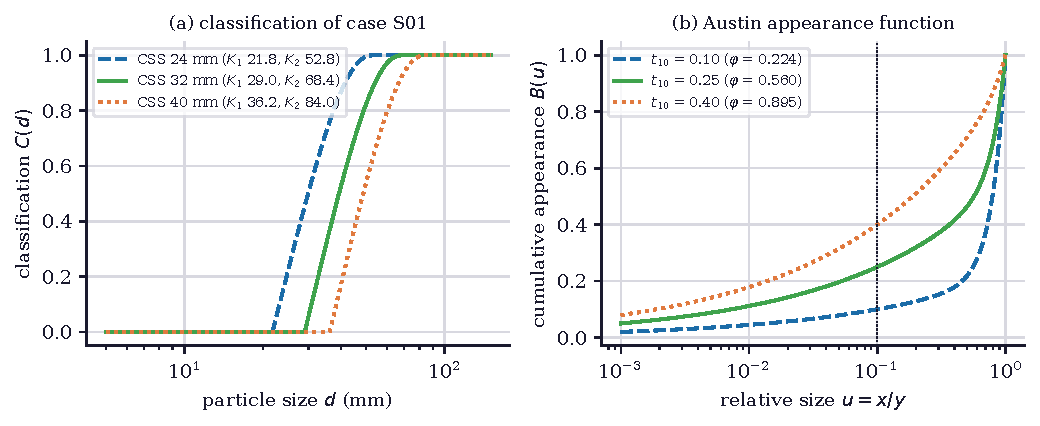
\includegraphics[width=\textwidth]{fig-chamber.pdf}
\caption{The two functions of the chamber, computed with the product's engine code: (a) the classification $C(d)$ of the secondary
case S01 at settings of $24$, $32$ and $40$~mm with the resulting $K_1$ and $K_2$; (b) the Austin appearance function at $t_{10}$ of
$0.10$, $0.25$ and $0.40$, each passing through $B=t_{10}$ at $u=0.1$ (dotted).}
\label{fig:chamber}
\end{figure}

\subsection{The Whiten population balance}\label{sec:m-whiten}

\emph{Theory.} The chamber is one breakage zone~\cite{whiten1972,napier1996}. A particle of class $j$ entering the zone is selected for
breakage with probability $c_j$, and the progeny of a broken particle report to finer classes through $\mathrm B$. Let $\mathbf x$ be
the mass flow through the zone per unit of feed: it is the feed plus the progeny of everything selected, $\mathbf x=\mathbf f+\mathrm
B\mathrm C\mathbf x$, and the product is the part of the flow that was not selected, $\mathbf p=(\mathrm I-\mathrm C)\mathbf x$. Hence
\begin{equation}
\mathbf p = (\mathrm I - \mathrm C)\,(\mathrm I - \mathrm B\mathrm C)^{-1}\,\mathbf f .
\label{eq:whiten}
\end{equation}
Because $\mathrm B$ is strictly lower triangular and $\mathrm C$ is diagonal, $\mathrm B\mathrm C$ is strictly lower triangular, so
$\mathrm M=\mathrm I-\mathrm B\mathrm C$ is unit lower triangular with determinant one and is never singular. Mass is conserved in exact
arithmetic: summing the balance and using $\mathbf 1^{\top}\mathrm B=\mathbf 1^{\top}$ on the columns that have finer classes gives
$\mathbf 1^{\top}\mathbf p=\mathbf 1^{\top}\mathbf f$, except for mass selected in the finest class, which has no finer class to go to;
the engine reports the closure $|\mathbf 1^{\top}\mathbf p-\mathbf 1^{\top}\mathbf f|$ before it renormalises the product. The same
balance gives the expected number of breakage events per unit of feed,
\begin{equation}
\nu = \mathbf 1^{\top}\mathrm C\,\mathbf x = \sum_{k} c_k x_k ,
\label{eq:nips}
\end{equation}
the quantity that Section~\ref{sec:validation} uses to check the solve against a particle-replacement walk.

\emph{Numerical scheme.} The inverse is never formed. Algorithm~\ref{alg:whiten} builds $\mathrm M$, solves $\mathrm M\mathbf x=\mathbf f$
by LU decomposition with partial pivoting (ported from the TypeScript engine as written, so both languages run the same operations),
applies $(\mathrm I-\mathrm C)$ with a floor at zero, records the closure, and renormalises. A conditioning proxy, the ratio of the
largest to the smallest absolute row sum of $\mathrm M$,
\begin{equation}
\kappa = \frac{\max_i \sum_j |M_{ij}|}{\min_i \sum_j |M_{ij}|},
\label{eq:cond}
\end{equation}
is kept for the regime near choke, where many entries of $\mathbf c$ approach one; a point with $\kappa$ above $10^{6}$ or not finite is
flagged ill-conditioned and marked invalid. At case S01 the proxy is $1.517$ and the closure $3.3\times10^{-16}$. Pivoting is
redundant for a unit triangular matrix but is kept so that the two engines stay identical for any input.

\begin{algorithm}[!t]
\caption{The Whiten solve of one operating point, as \texttt{whiten\_solve} runs it.}
\label{alg:whiten}
\begin{algorithmic}[1]
\Require classification $\mathbf c\in[0,1]^K$, breakage matrix $\mathrm B$ (strictly lower triangular, columns summing to one), feed $\mathbf f$ with $\mathbf 1^{\top}\mathbf f=1$
\Ensure product $\mathbf p$ with $\mathbf 1^{\top}\mathbf p=1$, mass closure $\epsilon$, conditioning proxy $\kappa$
\For{$i=1$ \textbf{to} $K$, $j=1$ \textbf{to} $K$}
  \State $M_{ij}\gets [i=j] - B_{ij}\,c_j$ \Comment{$\mathrm M=\mathrm I-\mathrm B\mathrm C$}
\EndFor
\State $\kappa \gets \max_i\sum_j|M_{ij}| \,/\, \min_i\sum_j|M_{ij}|$
\State factor $\mathrm P\mathrm M=\mathrm L\mathrm U$ by Gaussian elimination with partial pivoting \Comment{a zero pivot returns $\mathbf f$ and $\kappa=\infty$}
\State solve $\mathrm L\mathbf z=\mathrm P\mathbf f$ forward, then $\mathrm U\mathbf x=\mathbf z$ backward
\For{$i=1$ \textbf{to} $K$}
  \State $p_i\gets\max\!\left(0,\ (1-c_i)\,x_i\right)$
\EndFor
\State $\epsilon\gets\left|\sum_i p_i - \sum_i f_i\right|$ \Comment{reported before renormalising}
\State $\mathbf p\gets\mathbf p/\sum_i p_i$
\State \Return $\mathbf p,\ \epsilon,\ \kappa$
\end{algorithmic}
\end{algorithm}

\emph{Reading the solution.} Because $\mathrm M$ is unit lower triangular, the system $\mathrm M\mathbf x=\mathbf f$ is also solved by
forward substitution from the coarsest class down, $x_i = f_i + \sum_{j<i}B_{ij}\,c_j\,x_j$: the flow through class $i$ is its own feed plus the
progeny of everything broken in the coarser classes. This makes the physical reading of the balance explicit, and it is the recursion that the
particle-replacement check of Section~\ref{sec:val-walk} samples. At S01 the expected number of breakage events per unit of feed,
Equation~\eqref{eq:nips}, is $0.886$: a tonne of feed undergoes on average less than one nip in this model, because the half of the feed finer
than about $64$~mm is broken only in part and everything below $29$~mm passes unbroken. The product of S01 has $P_{80}=27.7$~mm, $P_{50}=12.1$~mm and
$P_{20}=1.83$~mm, a reduction ratio of $4.55$, and $15.0\%$ of its mass passes $1$~mm.

\emph{Cost.} Building $\mathrm M$ and the proxy are $O(K^2)$; the factorisation is $O(K^3)$, about $2K^3/3\approx1.5\times10^{4}$
floating-point operations for $K=28$; the two triangular solves are $O(K^2)$. One full evaluation of the engine, with the feed, both
functions, the solve, the readouts, the capacity, the power and the checks, takes a median of $\resEngineMed$~ms in Python
(Section~\ref{sec:arch-engine}).

\emph{Assumptions and limits.} One breakage zone, steady state, no spatial resolution of the chamber, no wear and no segregation. The
balance is the fast approximation of what a discrete-element simulation resolves particle by particle, and it inherits none of that
method's mechanism: its classification and breakage functions are inputs, not results.

\emph{Implementation and tests.} \texttt{model/\allowbreak{}crusher/\allowbreak{}whiten.py} (\texttt{whiten\_solve}, \texttt{assemble\_chamber},
\texttt{replacement\_walk}), \texttt{model/\allowbreak{}crusher/\allowbreak{}linalg.py} (\texttt{solve\_lu}, \texttt{cond\_proxy}) and
\texttt{model/\allowbreak{}crusher/\allowbreak{}engine.py} (\texttt{evaluate}), which runs the steps in order: the feed and its $F_{80}$; $K_1$, $K_2$, $K_3$ and
$\mathbf c$; the energy, $t_{10}$, $\varphi$ and $\mathrm B$; the solve; $P_{80}$, $P_{50}$, $P_{20}$ and the readouts; the throughput
and the power; the nip angle, the regime, the validity flags and the envelope codes. The acceptance criteria are mass closure with a
product finer than the feed and a finer product at a tighter setting (\texttt{test\_whiten\_solve\_conserves\_mass\_and\_product\_normalizes},
\texttt{test\_tighter\_css\_gives\_a\_finer\_product}).

\subsection{Capacity: a reduced Evertsson flow model}\label{sec:m-capacity}

\emph{Theory.} The capacity of a cone crusher rises with eccentric speed up to an optimum and falls past it: at low speed the chamber
discharges slowly, and past the optimum the gyrating head obstructs the free fall of the material faster than gravity clears it. The
flow model of Evertsson~\cite{evertsson1999,evertsson2000} resolves this in the chamber; the engine uses a reduced parametric form that
keeps the hump and the dependence on the discharge gap,
\begin{equation}
Q = \max\!\left(0,\ Q_{ref}\;\frac{s + T/2}{g_{ref}}\;\sigma_N\,e^{\,1-\sigma_N}\right),\qquad \sigma_N = \frac{N}{N_{opt}} .
\label{eq:capacity}
\end{equation}
The factor $\sigma_N e^{1-\sigma_N}$ has its maximum value one at $\sigma_N=1$ and is unimodal, and the opening factor is proportional
to the mean discharge gap $s+T/2$. The derivative of the hump factor, $(1-\sigma_N)e^{1-\sigma_N}$, is positive below the optimum and
negative above it, so a case run past the optimum speed loses capacity as the speed rises. Figure~\ref{fig:sweeps}(a) shows the speed
sweeps of the secondary cases S01 (at the optimum, $643$~t/h), S02 (below it) and S03 (past it, where capacity falls with speed).

\emph{Sensitivities.} The elasticities of the capacity with respect to its levers follow from Equation~\eqref{eq:capacity} inside the
positive range,
\begin{equation}
\frac{N}{Q}\frac{\partial Q}{\partial N} = 1 - \sigma_N,\qquad
\frac{s}{Q}\frac{\partial Q}{\partial s} = \frac{s}{s+T/2},\qquad
\frac{T}{Q}\frac{\partial Q}{\partial T} = \frac{T/2}{s+T/2},
\label{eq:elasticity}
\end{equation}
so one percent more speed gives $1-\sigma_N$ percent more capacity: a gain below the optimum, nothing at it and a loss past it. At S01
($\sigma_N=1$) the speed elasticity is zero; at S02 ($300$~rpm, $\sigma_N=0.833$) it is $+0.17$, and at S03 ($470$~rpm, $\sigma_N=1.306$) it is
$-0.31$, which is the falling side of the hump that the case is built to show. The setting and throw elasticities add to one: at S01 they are
$32/47=0.68$ and $15/47=0.32$. The speed sweep of S01 checks the closed form: at half the case speed ($\sigma_N=0.5$) the factor is
$0.5\,e^{0.5}=0.824$ and the trace gives $530$~t/h, and at $1.5$ times it the factor is $1.5\,e^{-0.5}=0.910$ and the trace gives $585$~t/h, both
equal to $643.16$~t/h times the factor. The power sweep of the same case has its maximum at a higher speed, because the specific energy of
Equation~\eqref{eq:t10} also grows with speed and makes the product finer (Section~\ref{sec:m-breakage}).

\emph{Parameters and how they were set.} Table~\ref{tab:machines} gives $Q_{ref}$, $N_{opt}$ and $g_{ref}$ per class: for the secondary
cone $520$~t/h, $360$~rpm and $38$~mm, so S01 (setting $32$~mm, throw $30$~mm, $360$~rpm) gives $520\times47/38=643.16$~t/h. The circuit
values are illustrative of their class; only the shape (unimodal in speed, increasing in setting and throw) is claimed for them. On the
calibrated lane $Q_{ref}$ is replaced by $Q_T=647$~t/h, the number Rocha et al.\ give as the capacity of the HP500 in the base case
of the vendor's simulator (granite, work index $16$~kWh/t, feed $f_{80}$ of $100$~mm, setting $38$~mm, medium cavity), where it is
the base of a different, multiplicative throughput model (Section~\ref{sec:m-hp500})~\cite{rocha2024}. Put into
Equation~\eqref{eq:capacity} it means something else: at the base-case setting of $38$~mm, the HP500 throw of $34$~mm and the
optimum speed, the reduced form gives $647\times(38+17)/38=936$~t/h, not $647$~t/h. CrusherCal refits this scalar per fold and
CrusherBayes samples it, so the engine's throughput on the surveys does not rest on its published value.

\emph{Cost and numerical scheme.} A closed form, $O(1)$; the floor at zero keeps the throughput non-negative for any input.

\emph{Assumptions and limits.} No cavity-level material balance, no feed segregation, no choke-level dynamics: the reduced form is the
hump and the gap dependence. It is not a vendor capacity table. The throughput of a survey is set by the plant together with the
setting, so the capacity model is a prediction of the feed rate only under the assumption that the machine runs at its capacity. On the ten
surveys that assumption holds to first order: the measured feed rate rises with the setting at about $32$~t/h per millimetre
(Figure~\ref{fig:surveys}), and the capacity factor of the calibrated engine, with no other information than the setting, reproduces the
measured feed rates to $11.55\%$ in sample (Section~\ref{sec:m-hp500}). A plant that runs a crusher below its capacity, for example when the
feed is restricted upstream, breaks the assumption, and the capacity is then an upper bound of the throughput rather than a prediction of it.

\emph{Implementation and tests.} \texttt{model/\allowbreak{}crusher/\allowbreak{}capacity.py} (\texttt{CAP}, \texttt{HP500\_QREF}, \texttt{throughput},
\texttt{optimal\_speed}). The acceptance criterion is a capacity unimodal in speed (\texttt{test\_capacity\_is\_unimodal\_in\_speed}); a
second test requires a positive and finite throughput and power at every valid point. Each trace carries a sweep of $31$ speeds from
$0.5$ to $1.5$ times the case speed.

\begin{figure}[!t]
\centering
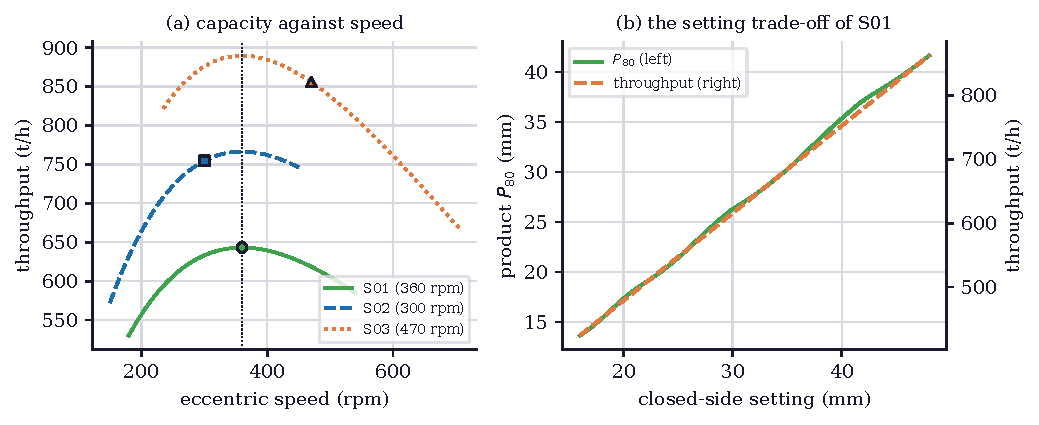
\includegraphics[width=\textwidth]{fig-sweeps.pdf}
\caption{The engine's response to two levers, read from the committed traces: (a) throughput against eccentric speed for the secondary
cases S01, S02 and S03, with each case's operating speed marked and the optimum of $360$~rpm dotted; (b) product $P_{80}$ and
throughput of S01 against the closed-side setting.}
\label{fig:sweeps}
\end{figure}

\subsection{Regimes and the nip angle}\label{sec:m-regimes}

\emph{Theory.} Two outputs qualify a result rather than compute a product: the regime of the operating point and the nip angle against
its grip limit. A setting at or above the feed's $80\%$ passing size grips little of the feed, and a setting at or above its top size
grips none of it; in both cases the population balance would still return a product, and the engine must say that the number means
little. The nip angle of a compression crusher is the angle between the two crushing surfaces at the point where a particle is gripped;
a particle is nipped when the angle is at most twice the friction angle, the grip limit,
\begin{equation}
\alpha = \alpha_0 + 3\left(\frac{s}{g_{ref}} - 1\right),\qquad \alpha_{lim} = 2\arctan\mu_f,
\label{eq:nip}
\end{equation}
with $\alpha_0=22^\circ$ for the cones and the gyratory and $19^\circ$ for the jaw, and $\mu_f=0.35$, so $\alpha_{lim}=38.58^\circ$. The
limit follows from a force balance on a particle squeezed between two surfaces that open at the angle $\alpha$: each surface pushes with a
normal force $F_n$ inclined by $\alpha/2$ from the closing direction, and friction can hold at most $\mu_fF_n$ along each surface, so the
particle is held when $2\mu_fF_n\cos(\alpha/2)\ge2F_n\sin(\alpha/2)$, that is when $\tan(\alpha/2)\le\mu_f$. At case S01 the nip angle is
$21.53^\circ$, well inside the limit. Over the $27$ committed traces the angle ranges from $18.18^\circ$ (the jaw J02) to $41.11^\circ$ (the
invalid control CI1, whose setting of $280$~mm is more than seven times the reference gap); CI1 is the only case above the limit, and the next
largest is the pass-through control CP1 at $31.63^\circ$.

\emph{The rules, as the engine applies them.} With $F_{80}$ the feed size on the grid and $e_0=256$~mm the top edge, and $\rho=F_{80}/P_{80}$
the reduction ratio:
\begin{equation}
\text{regime} = \begin{cases}
\text{invalid}, & s \ge e_0,\\
\text{pass-through}, & F_{80}\le s < e_0 \ \text{ or }\ \rho < 1.05,\\
\text{choke}, & \text{otherwise},
\end{cases}
\label{eq:regime}
\end{equation}
and the point is marked invalid when $s\ge e_0$, when the conditioning proxy exceeds $10^{6}$ or is not finite, or when the envelope
check finds an implausible input (Section~\ref{sec:m-envelope}). Each rule writes a stable flag code into the manifest
(\texttt{pass\_through}, \texttt{css\_ge\_feed\_top}, \texttt{negligible\_reduction}, \texttt{ill\_conditioned}), which the web maps to
text in both languages and refuses when it does not know the code. Two sourced warnings, the setting below the vendor minimum of the
machine class and a reduction ratio above the typical ceiling of one stage, never change the regime or the validity (their bounds are in
Section~\ref{sec:m-envelope}). The regime type also lists \emph{trickle}, which the engine never assigns. Among the $27$ committed traces,
$23$ are choke, three pass-through (CP1, G02 and the survey HP500-03, whose measured $f_{80}$ of $47$~mm is below its setting of
$48$~mm) and one invalid (CI1).

\emph{Parameters and how they were set.} $\alpha_0$ and $\mu_f$ are typical values, not a vendor's; the factor $3$ (half of $6^\circ$
per unit of relative gap) makes the angle rise modestly with the setting. The thresholds $1.05$ on the reduction ratio and $10^{6}$ on
the proxy are the engine's. The nip angle is reported and drawn in the chamber view; it does not set the regime.

\emph{Cost.} $O(1)$ comparisons after the solve.

\emph{Assumptions and limits.} \emph{Choke} is the label when no rule fires; it is not a choke-feed model. The rules are not a safety
check of a real machine. The pass-through rule compares the setting with the feed's $F_{80}$ on the grid, so a coarse feed whose grid value
is truncated (Section~\ref{sec:m-feed}) can sit on either side of the rule depending on the grid. The survey HP500-03 is a fine feed:
its grid $F_{80}$ of $47.15$~mm and its measured $f_{80}$ of $47$~mm both lie just below its setting of $48$~mm, so the rule fires on
either value.
In both cases the engine still returns a product, flagged, and the manifest records the codes \texttt{pass\_through} and \texttt{f80\_lt\_css};
the web shows the flags beside every number of such a case and never presents it as a confident answer.

\emph{Implementation and tests.} \texttt{model/\allowbreak{}crusher/\allowbreak{}engine.py} and \texttt{model/\allowbreak{}crusher/\allowbreak{}capacity.py} (\texttt{nip\_angle},
\texttt{nip\_limit}); the flag codes are in \texttt{core/\allowbreak{}manifest.py}. The acceptance criterion is that the pass-through and invalid
flags fire at a setting at or above the feed's $F_{80}$ and top size
(\texttt{test\_pass\_through\_and\_invalid\_guard\_fires\_when\_css\_ge\_feed\_top\_size}); the controls CP1 and CI1 are baked to carry
them.
